\documentclass[12pt]{article}

\usepackage[utf8]{inputenc}
\usepackage[brazil]{babel}
\usepackage{amsmath,amssymb}
\usepackage{pdfsync}
\usepackage[all]{xy}
\usepackage{color}
\usepackage{hyperref}
\usepackage{graphicx}
\usepackage[ruled,vlined]{algorithm2e}
\usepackage{amsthm}

\newtheorem{theorem}{Teorema}[section]
\newtheorem{corollary}{Corolário}[theorem]
\newtheorem{lemma}[theorem]{Lema}

\title{{\large Universidade de Brasília \\ Instituto de Ciências Exatas \\
Departamento de Ciência da Computação} \\[1cm]
117536 - Projeto e Análise de Algoritmos Turma: B\\[.5cm]
Análise Assintótica e Corretude do Algoritmo KMP Utilizando PVS}
\author{Gabriel Levi - 16/0006490 \\
        Gabriel Nunes - 16/0006597}
\date{\today}

\begin{document}
\maketitle
\newpage

\section{Introdução}
\noindent A verificação formal de algoritmo, no que tange ao seu comportamento assintótico e a corretude do algoritmo é interesse
central da Ciência da Computação. Por vezes, a prova via argumentação, isto é, lápis e papel pode ser suficiente para que o escritor
convença o leitor de que o algoritmo está correto. Contudo, esse modelo de prova se sustenta muita vezes em passos de pura intuição,
assumições que ambas as partes enxergam como um axioma, e saltos lógicos que por mais naturais que pareçam escondem um conjunto não-trivial
de conceitos. A ocorrência desses aspectos em uma formalização pode ocultar falhas que, de fato, provem a incorretude do algoritmo e desmonstre
um comportamento assintótico pior do que o esperado.

Como forma de minimizar o exposto anteriormente, introduz-se os sistemas de verificação de provas. Os verificadores garantem que os passos realizados
dentro de uma prova respeitem o conjunto de regras de sua lógica intrínseca. Então, dadas premissas corretas e um ponto factível onde se deseja chegar, qualquer
passo intermediário tem que, necessariamente, estar correto. Obviamente, construções ruins de objetivos e premissas podem levar a provas, ainda sim, incorretas
ou impossíveis. Podemos concluir então que os sistemas de verificação pressupõe que uma prova, ou pelo menos a ideia da mesma, já exista e o usuário interessado
o utilize para demonstrar que de fato aquela construção vale.

Um dos verificadores, PVS - Prototype Verification System - é a linguagem de especificação e provador automatizado de teoremas que aqui será utilizado.
PVS trabalha com implementações em distribuições de diferentes versões de LISP. Em um arquivo, o usuário define premissas - um algoritmo - e teoremas.
O arquivo é dado como entrada para o provador que requisita as regras a serem aplicadas até que o teorema desejado seja provado. As regras reconhecidas pelo
PVS tratam-se simplesmente de regras da lógica de primeira-ordem. O PVS permite também que uma prova possa ser revisitada em uma representação gráfica que
revela cada passo bem como suas depedências.

O objetivo deste trabalho é analisar assintóticamente o custo de tempo e a corretude do algoritmo de ordenação \textit{Merge Sort} via PVS. O Merge Sort foi criado
em meados de 1945 por John Von Neumann. A escolha deste algoritmo se deu por ser de implementação muito simples para múltiplas estruturas de dados tais como
vetores e listas ligadas e por, ainda sim, ser um algoritmo com múltiplas aplicações dado o seu custo de execução. Este relatório apresentará a ideia de prova
formalizada via provador e fica a critério do leitor visitar o repositório para verificar a mesma. A formalização completa pode ser encontrada em \url{github.com/paa-2019-2/levi-nunes}.

Esse documento se organizará, daqui em diante, por um capítulo \ref{explaining} de revisão teórica. Em seguida, no capitulo \ref{merge_sort}, a apresentação do algoritmo Merge Sort. 
O capitulo \ref{complexity} apresentará a ideia abordada pelos autores para a análise de assintótica do algoritmo
bem como argumentação sobre o pior e o melhor caso do mesmo. O capitulo \ref{correctness} apresentará, como o capitulo anterior, a ideia abordada
e sua argumentação. Por fim, o capitulo de conclusão, apresentará um resumo dos resultados aqui encontrados acompanhado de um meta-texto discorrendo sobre
as principais dificuldades do trabalho com o verificador formal de provas.

\section{Revisão teórica}
\label{explaining}

Este capítulo apresentará conceitos importantes para o entedimento do que se segue nos capitulos posteriores. Caso sinta-se a vontade com o conceito, 
cujo o nome será enunciado no título de cada subseção, não há nenhum mal em pular. Cada um dos conceitos será apresentado de maneira simples mais preocupado
com ser inteligível para o leitor do que com um profundo formalismo. Em compensação, uma boa bibliografia de apoio será indicada para aqueles interessados em 
se aprofundar ou que não acharam que o texto de uma ou mais subseções foi suficiente.

// Se não existir nada além de Notação Assintótica, converter pra uma seção de revisão sobre Notação assintótica.
\subsection{Notação assintótica}

\subsection{}

\section{O algoritmo Merge Sort}
\label{merge_sort}

O algoritmo fundamenta-se na técnica Dividir-para-Conquistar. A técnica consiste em, dada uma instância do problema
quebra-la em partes até que as mesmas sejam fáceis ou triviais de se resolver, por fim, cada pequena solução é combinada a fim
de obter a solução para o problema maior. Apesar de parecer similar, esta técnica é bem diferente de programação dinâmica pois
cada subproblema é disjunto dos demais. Desta forma, o algoritmo recebe uma lista como entrada uma lista de elementos comparáveis
e divide tal lista até que cada sublista possua tamanho unitário - trivialmente ordenável - e então combina as listas para obter
a lista de entrada ordenada. O processo pode ser visualizado na figura \ref{fig:merge_sort_example} onde a parte superior diz respeito
a dividir e a parte inferior diz respeito a conquista.

\begin{figure}[h]
        \centering
        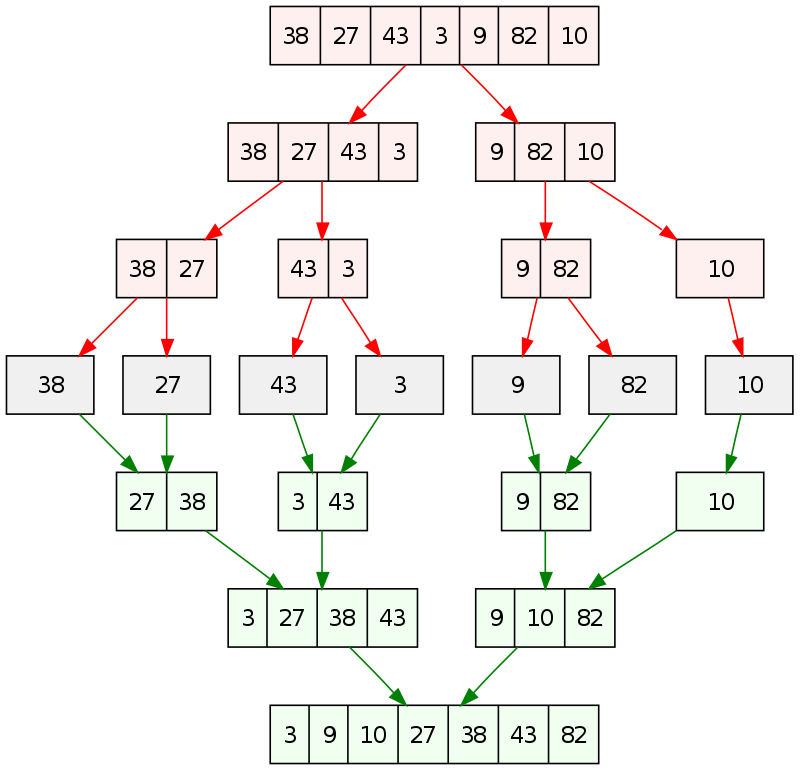
\includegraphics[width=0.7\textwidth]{figures/merge.png}
        \caption{Ordenação da instância [38, 27, 43, 3, 9, 82, 10]}
        \label{fig:merge_sort_example}
\end{figure}

Por mais poderosa que seja a ideia, a implementação do Merge Sort é bem simples e pode ser deduzida a partir do pseudo-código abaixo, 
para fins de facilitar a leitura, denotamos a cabeça da lista $\tau$ como $car(\tau)$ e a sua calda como $cdr(\tau)$, o operador $+$
significa inserção de um elemento no início de uma lista ou a concanetação de duas listas. 

\begin{algorithm}[H]
        \KwData{$\rho, \eta : Sorted\ lists $}
        \KwResult{Sorted merge of $\rho$ and $\eta$}
        \eIf{$\rho = Nil$ or $\eta = Nil$}{
            $\textbf{return}\  \rho + \eta$
        }{
            \eIf{$car(\rho) \leq car(\eta)$}{
                $\textbf{return}\ car(\rho) + MERGE(cdr(\rho) ,\ \eta)$
            }{
                $\textbf{return}\ car(\eta) + MERGE(\rho,\ cdr(\eta))$
            }
        }
        \caption{MERGE}
\end{algorithm}

\begin{algorithm}[H]
        \KwData{$\tau : List\ of\ comparable\ elements $}
        \KwResult{$Sorted\ permutation\ of\ \tau$}
        \eIf{$length(\tau) \leq 1$}{
                $\textbf{return}\ \tau$
        }{
                $prefix \leftarrow\ MERGESORT(first\_half(\tau))$\;
                $suffix \leftarrow\ MERGESORT(second\_half(\tau))$\;
                $\textbf{return}\ MERGE(prefix,\ suffix)$\;  
        }
        \caption{MERGESORT}
\end{algorithm}
\section{Análise assintótica do Merge Sort}
\label{complexity}

\section{Corretude do algoritmo Merge Sort}
\label{correctness}

A corretude de um algoritmo passa por demonstrar que o mesmo possui certas características independente da instância e que essas características
se verifiquem antes, durante e depois da execução. Para um algoritmo de ordenação, é esperado que o mesmo responda para qualquer entrada uma permutação
ordenada da mesma, isto é, a saída não só deve estar ordenada como também o número de ocorrências de cada elemento deve ser o mesmo da lista de entrada.

A análise de MERGESORT nos leva a uma série de resultados intermediários que fortalecem a argumentação da corretude do algoritmo. Tais resultados estão expostos
abaixo nesta seção e a formalização em PVS dos mesmos pode ser encontrado no repositório apresentado previamente na introdução deste texto.

\begin{lemma}
\label{merge-preserves-occurrences}
        Para quaisquer $\rho$ e $\eta$, listas, e $n$ valor, o número de ocorrências de $n$ em $MERGE(\rho,\ \eta)$ é igual ao número de ocorrências
        de $n$ em $\rho$ mais o número de ocorrências de $n$ em $\eta$.
\end{lemma}

\begin{proof}

\end{proof}

\begin{lemma}
\label{merge-preserves-length}
        Para quaisquer entradas $\rho$ e $\eta$, listas, o tamanho da lista resultante de $MERGE(\rho,\ \eta)$ é a soma
        dos tamanhos de $\rho$ e $\eta$.
\end{lemma}

\begin{proof}

\end{proof}

\begin{lemma}
\label{merge-is-permutation}
        Para quaisquer entradas $\rho$ e $\eta$, $MERGE(\rho,\ \eta)$ é uma permutação de concanetação de $\eta$ e $\rho$.
\end{lemma}
\begin{proof}
        
\end{proof}

\begin{lemma}
\label{merge-of-sorted-is-sorted}
        Para quaisquer entradas $\rho$ e $\eta$, se ambas as listas estão ordenadas então
        a resultante de $MERGE(\rho,\ \eta)$ também será uma lista ordenada. 
\end{lemma}

\begin{proof}
        Basta demonstrar que para qualquer iteração de $MERGE$, o menor elementos dentre ambas as listas é escolhido para inserção no final
        da lista parcialmente resultante. Uma vez que ambas as listas são ordenadas, necessariamente o menor elemento será a cabeça de $\rho$ ou de $\eta$.
        Utilizando da definição de $MERGE$ e induzindo sobre o tamanho de ambas as listas 3 situações emergem:
        \begin{enumerate}
                \item Alguma das listas $\rho$ e $\eta$ tem tamanho 0.
                \item A cabeça de $\rho$ é menor ou igual que a cabeça de $\eta$.
                \item A cabeça de $\rho$ é maior que a cabeça de $\eta$.
        \end{enumerate}

        Na primeira situação, no máximo uma das listas possui elementos, então o elemento tomado para a composição da lista resultante será a cabeça
        (o menor elemento) daquela que ainda não é vazia, por conveniência, o algoritmo já retorna a lista inteira, mas se de fato tivesse que escolher apenas
        um, seria o menor disponível. O segundo e o terceiro caso são similares, a cabeça de $\rho$ é igual ao menor elemento de $\rho$ e o mesmo vale para a cabeça
        de $\eta$, logo, o menor entre os ambos será o menor dentre todos e este será escolhido para a inserção ao final da lista resultante, a chamada recursiva 
        posterior cai novamente em algum dos 3 casos.

\end{proof}

\begin{lemma}
\label{mergesort-preserves-length}
        Para qualquer entrada $\tau$, lista, o tamanho de $\tau$ é igual ao tamanho de $MERGESORT(\tau)$.
\end{lemma}

\begin{proof}
        
\end{proof}

\begin{lemma}
\label{mergesort-is-permutation}
        Para qualquer lista $\tau$, a resultante de $MERGESORT(\tau)$ é uma permutação de $\tau$.
\end{lemma}

\begin{proof}
        
\end{proof}

\begin{lemma}
\label{mergesort-sorts}
        Para qualquer lista $\tau$, a resultante de $MERGESORT(\tau)$ é uma lista ordenada.
\end{lemma}

\begin{proof}
        
\end{proof}

\begin{theorem}
\label{mergesort-is-correct}
        Para qualquer lista $\tau$, a resultante de $MERGESORT(\tau)$ é uma permutação ordenada de $\tau$.
\end{theorem}

\begin{proof}
        
\end{proof}

\section{Conclusão}
\label{conclusion}

\bibliographystyle{acm}
\bibliography{reference}

\end{document}

%%% Local Variables:
%%% mode: latex
%%% TeX-master: t
%%% End:
